\documentclass[../main.tex]{subfiles}
\graphicspath{{\subfix{../figures/}}}
%
\title{建立思维框架}
%
\begin{document}
\maketitle
\section{为何建立思维框架}
很多人觉得建立思维框架即等同于限制思维,即等同于思维僵化。
确实思维应是不受限制的,但问题的关键并不在于要不要建立思维框架,
而是学会不用单一的思维方式去思考所有的问题。

建立多元的思维模型,学会用不同的角度、不同的方法去看待和解决问题,
我们才能不断提升自身的能力。

而且很多情况下我们面临的其实不是思维僵化,而是思维空白,
是面对难题无从下手的窘境。在这种情况下,积累一些想问题的思路和方法,
可以让你快速找到突破口,从各个角度把事情想得清楚明白。
%
\section{如何建立思维框架}
大脑其实和肌肉类似,是越练越快的。可是大部分人其实没有思考的自觉性,
我们生活在持续的混沌之中。因而,有意识地多做思维练习,
在日常工作和生活中多思考,多总结,多问问题。

积累得多了,就可以慢慢建立起一套适用于自己的思维框架。
思考的技能是后天习得,
学会如何思考其实是每个人在每个阶段都应该学习和掌握的。
\\

\begin{cuenotes}
  \cue{几个思考的原则}
  \note{
    \textbf{决策时,尽可能全面地收集决策相关信息}: \\
    去哪个大学,选择什么专业,选择什么行业,从事什么工作,
    是否要跳槽,去哪个城市…尽可能全面地收集相关信息,
    从而才能做出更优的决策。
  }
  \note{
    \textbf{保持批判,质疑一切主张,包括自己的想法}: \\
    人类有很强的自我欺骗能力,
    我们很擅长为自己先入为主的想法寻找各种证据。
    因而,仔细检查自己思考的逻辑,可以识别自身想法的漏洞和缺陷。
  }
  \note{
    \textbf{虚心聆听别人的看法,善于引入外部意见}: \\
    认识到别人的错误比认识到自己的错误要容易得多。
    在做重大决策时,多听听他人的意见和批评。
  }
  \note{
    \textbf{保持专注,将注意力集中在思考的问题和目标上}: \\
    专注力是一种稀缺资源,当你在思考时,
    尽量克服那些分散或干扰我们注意力的因素,
    能让你更快更有效地进行思考。
  }
  \cue{锻炼思维的有效方式}
  \note{
    \textbf{自由头脑风暴}: \\
    聚焦在一个问题或者争议上,尽可能地进行发散,
    写下你所有能想到的东西。先不加评判,
    在发散完成后再进行逻辑的重组和整理,形成完整的看法和见解。
  }
  \note{
    \textbf{清单式思考}: \\
    当你不知道当下要做什么的时候,可以列出一份待做事项的清单,
    列出所有要做的事情并界定每件事的处理次序和时间范围,
    然后一件一件把它们解决掉。
  }
  \note{
    \textbf{写文章或或即兴演讲}: \\
    写作需要有中心思想,更需要逻辑来论证你的观点。
    当你尝试去表达,去自圆其说,思维即被激发。
    从提出结论到论证结论,需要完整的逻辑和清晰的表达。
    锻炼信息的传达能力,也是在锻炼思维。
  }
\end{cuenotes}
%
\section{行之有效的思维框架}
所谓思维框架,其实就是思考问题的思路和方法。
积累尽量多的框架,有助于我们建立起多元的思维模型,
能从多个角度去思考和解决问题。
%
\subsection{逆向思维法}
我们总是集中精力在想``如何成功'',
但有时想想为什么会失败可能更容易找到做对事情的方法。
预先设想惨败结果,分析可能的原因,并尽量避免。
``减少错误''有时候比``追求''正确有效得多。

举个例子: 要想过得开心,可以想想是什么让你不开心。

另外,当你百思不得其解时,向上溯源思考为什么自己会产生这样的问题,
会找到更本质的原因。因为向上消解问题是一个很好的逆向思维的方式。
%
\subsection{SWOT 分析法}
SWOT分析是将各种主要内部优势、劣势和外部的机会和威胁等,
通过调查列举出来,并依照矩阵形式排列,然后用系统分析的思想,
把各种因素相互匹配起来加以分析,从中得出结论。
%
\begin{itemize}
  \item S(strengths)优势
  \item W(weaknesses)劣势
  \item O(opportunities)机会
  \item T(threats)威胁
\end{itemize}
%
\begin{figure}[H]
  \begin{center}
    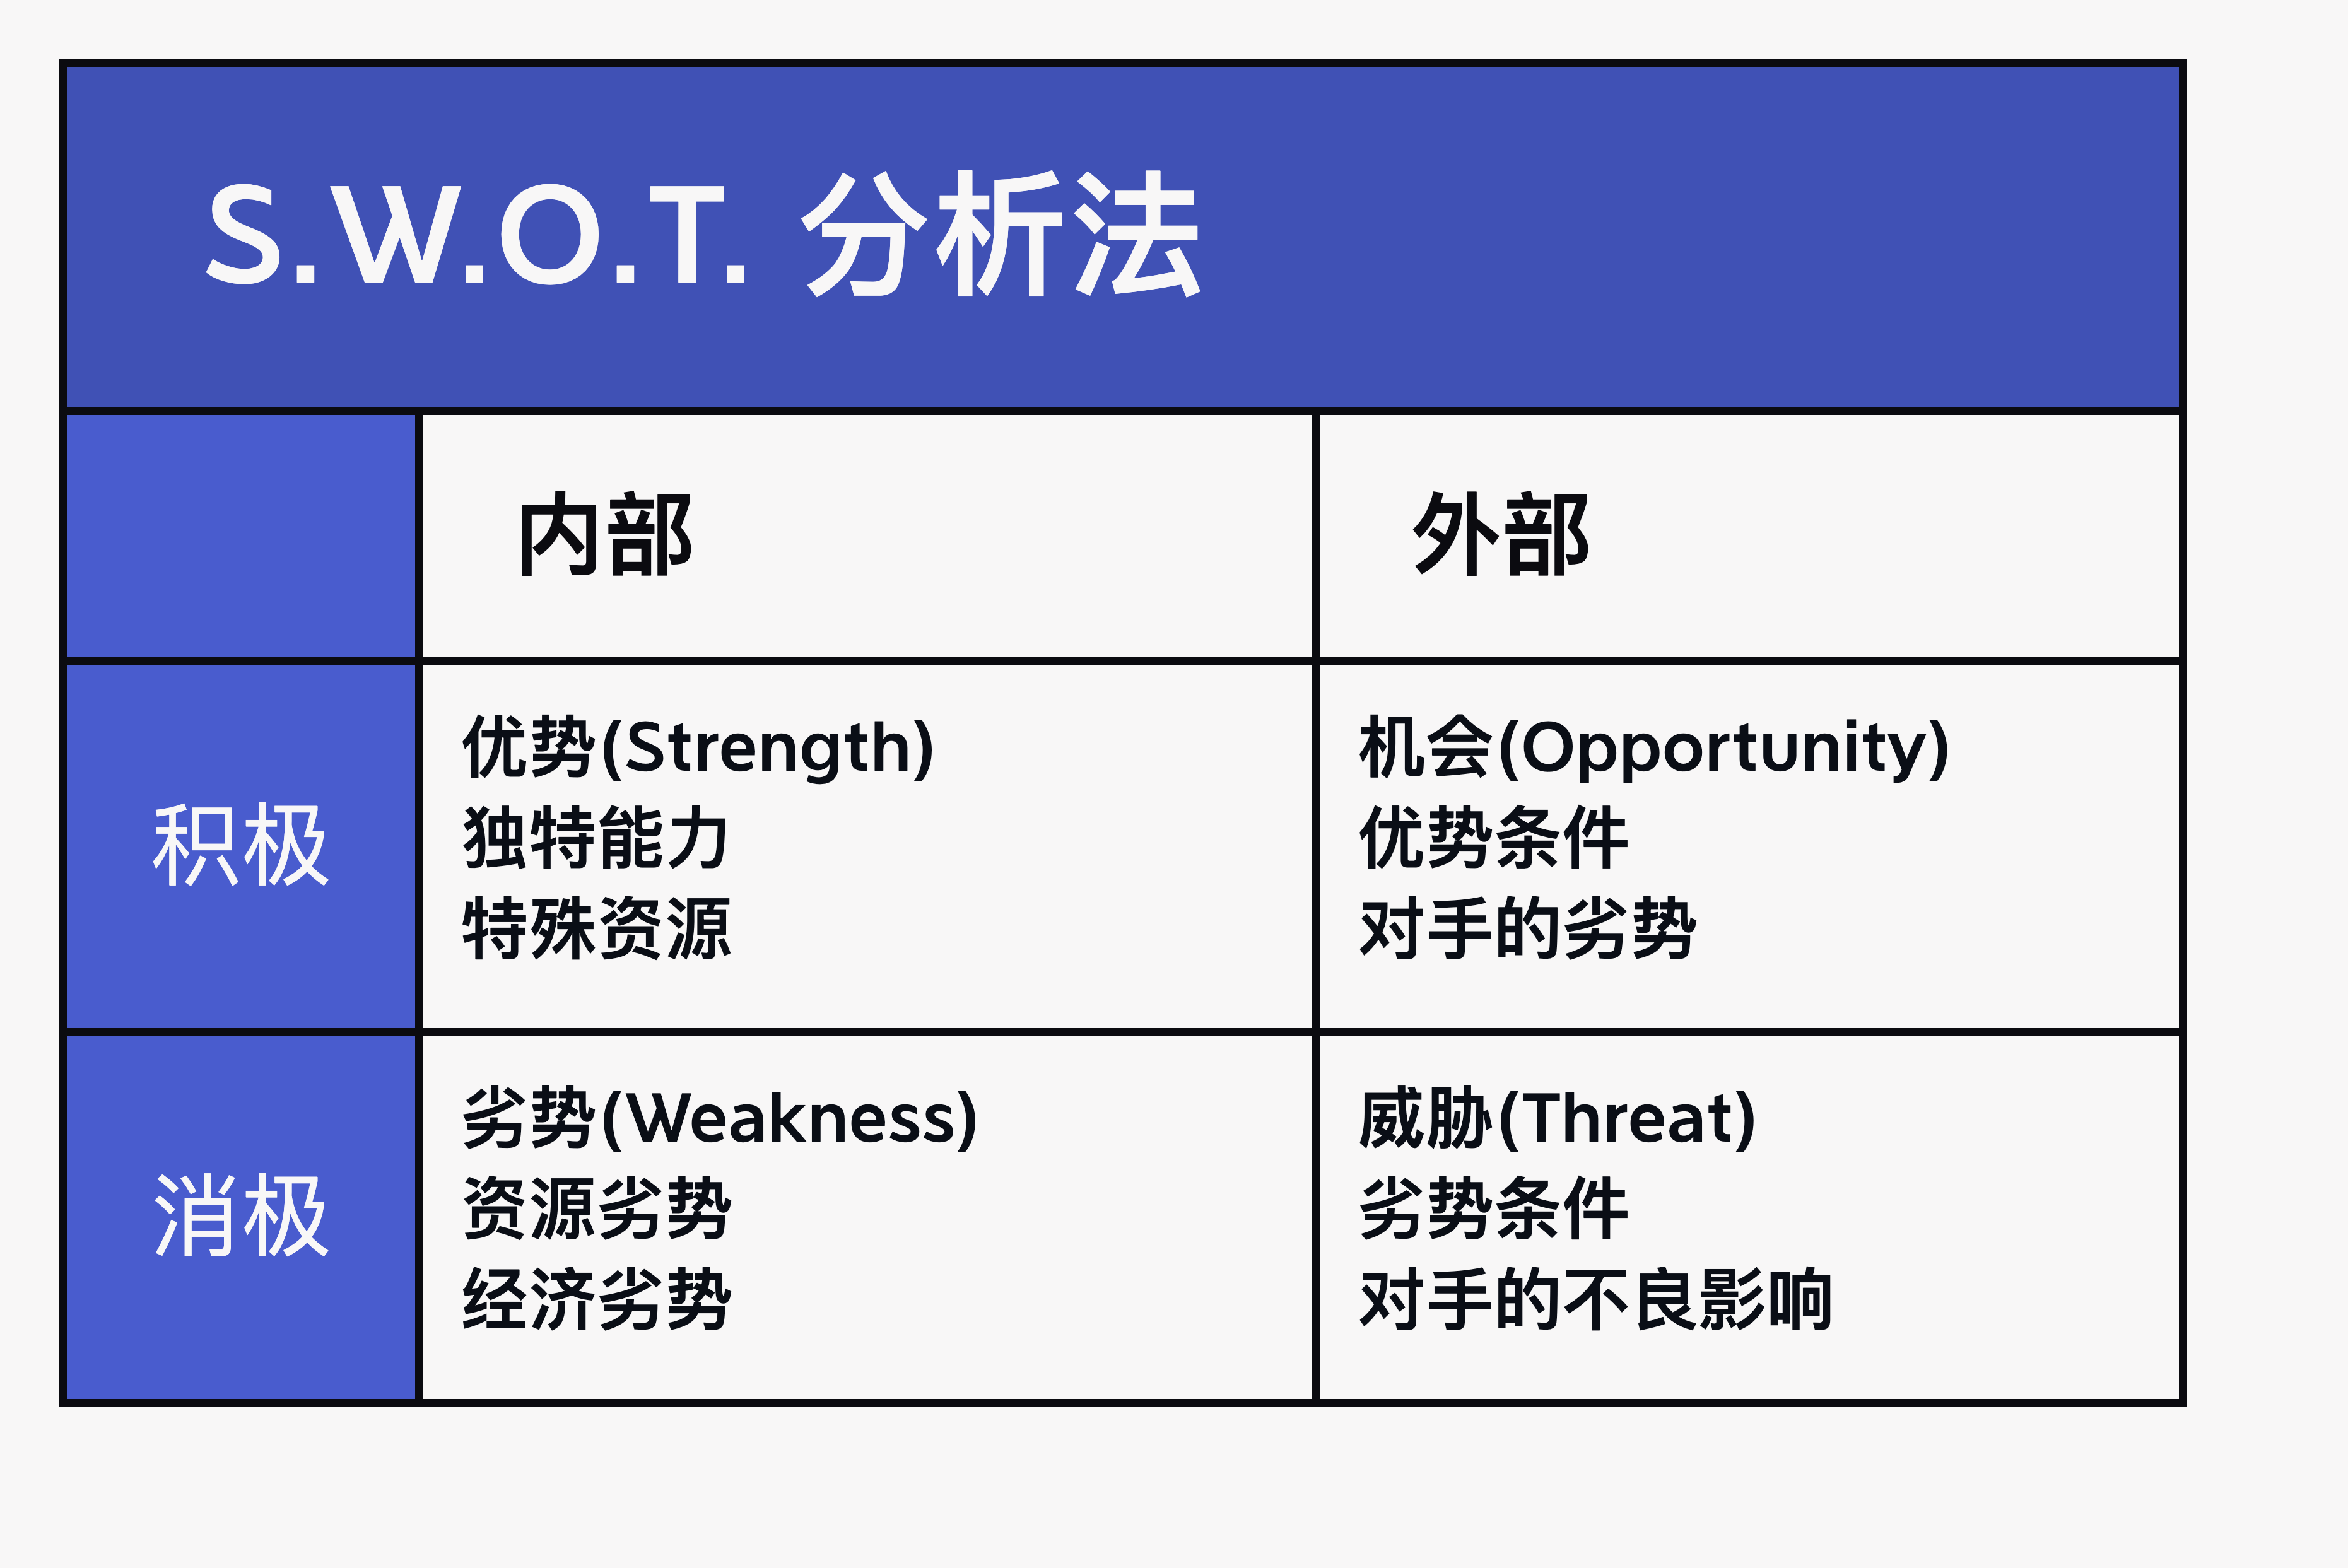
\includegraphics[width=0.50\textwidth]{swot.png}
  \end{center}
  \caption{SWOT分析法}
\end{figure}
%
运用这种方法,可以对研究对象所处的情景进行全面、系统、准确的研究,
从而根据研究结果制定相应的发展战略、计划以及对策等。
%
\subsection{因果分析法(鱼骨图)}
鱼骨图又被称为``因果分析图'',是一种发现问题``根本原因''的有效方法。
通过对问题的层层拆解,我们可以从表面的现象深挖问题的本质。
我们可以用它来进行事件分析、因果分析、问题分析等。
%
\begin{figure}[H]
  \begin{center}
    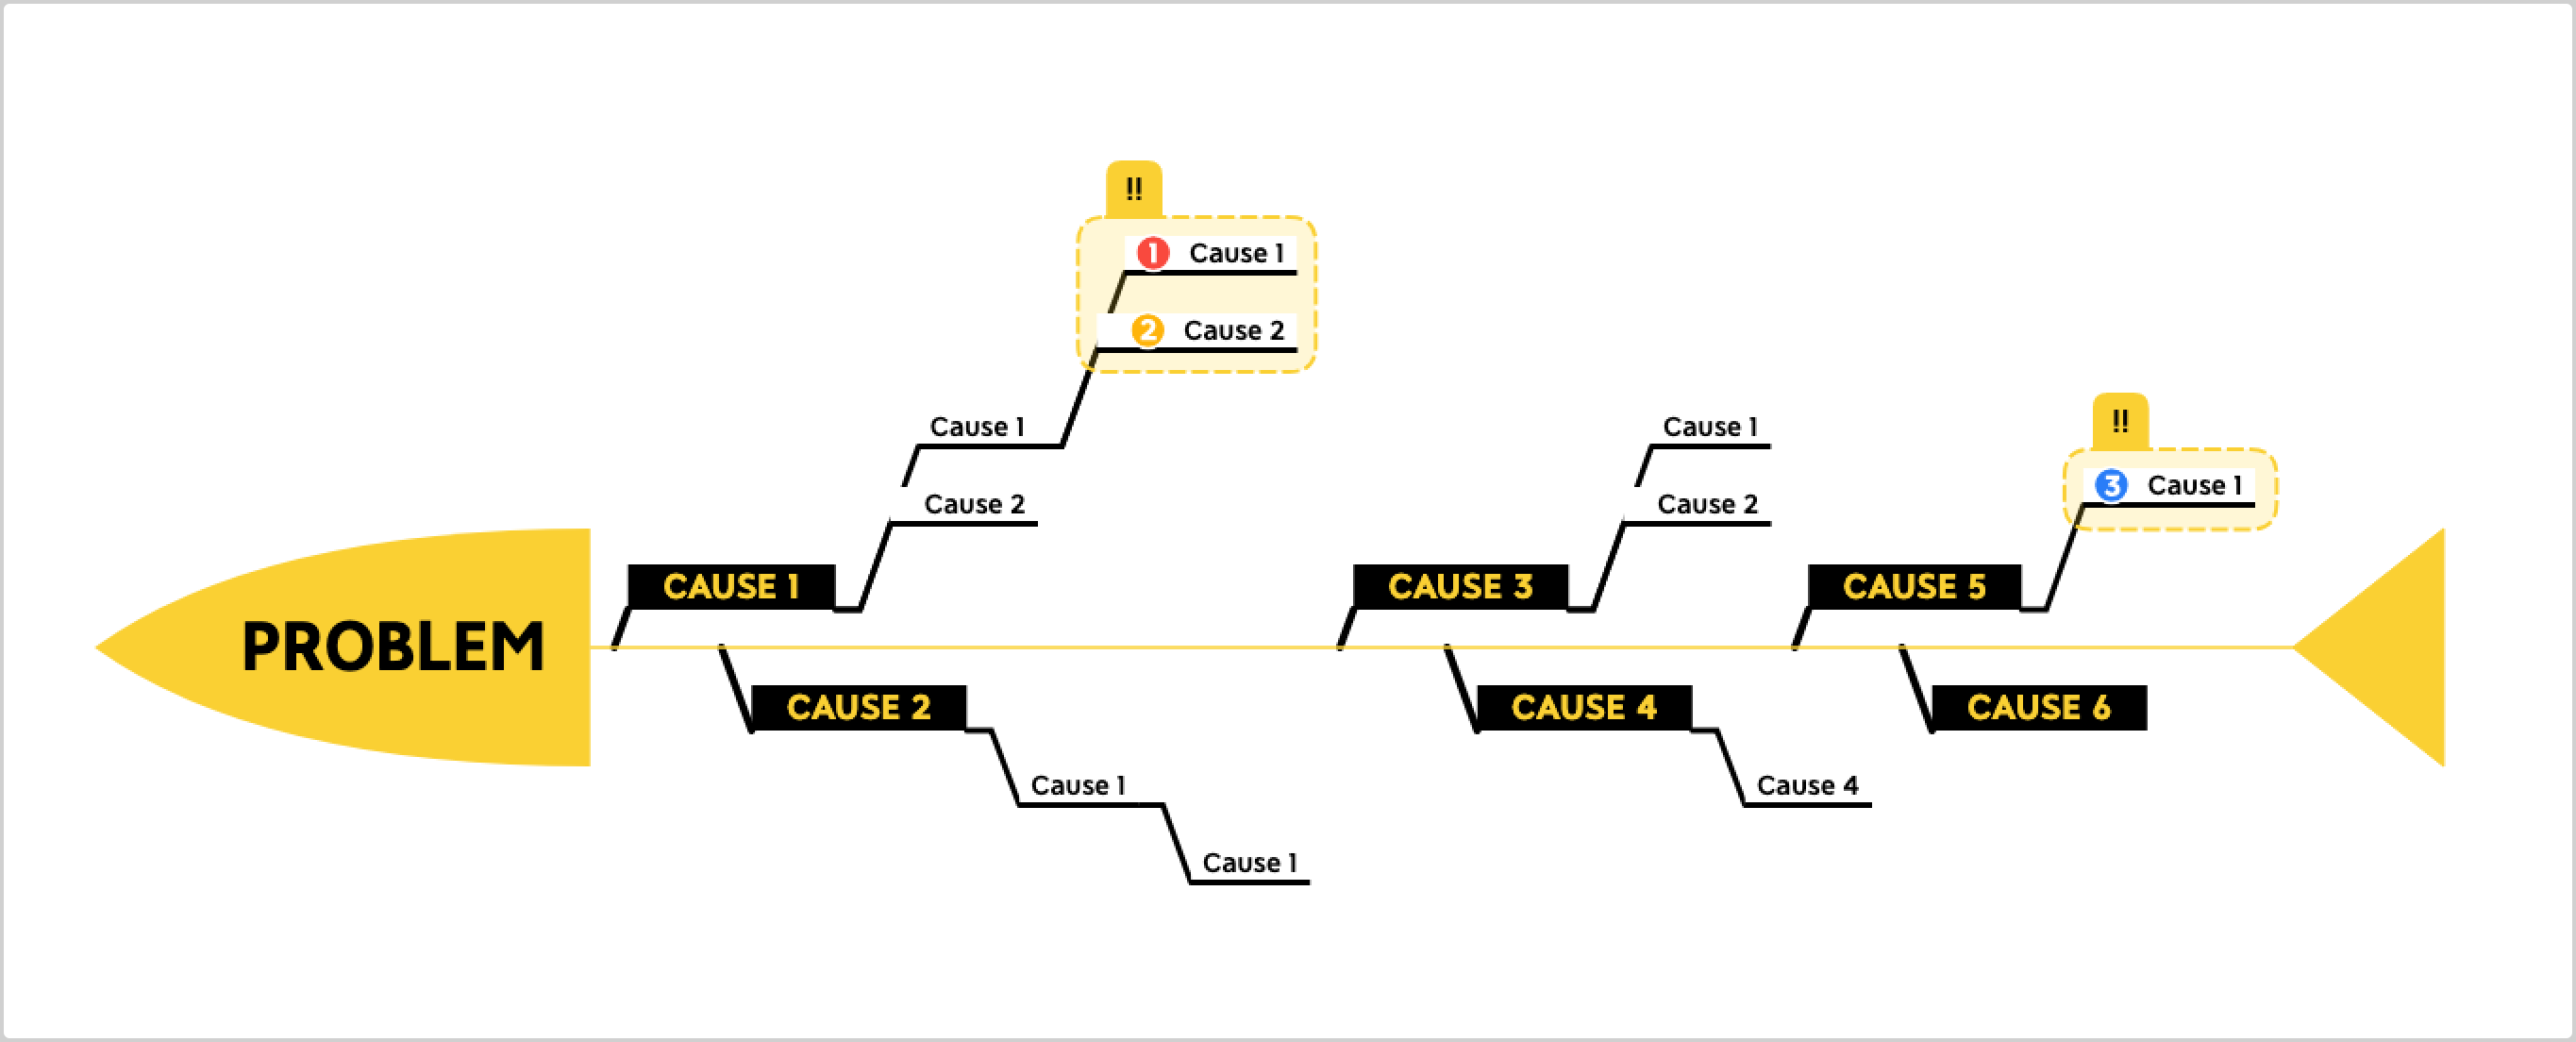
\includegraphics[width=0.80\textwidth]{鱼骨图.png}
  \end{center}
  \caption{鱼骨图}
\end{figure}
%
\textbf{鱼骨图绘制步骤}:
\begin{enumerate}
  \item 明确要解决的问题,将问题写在鱼骨头;
  \item 从各个角度进行思考,找出各个问题;
  \item 对问题进行分类,分组在鱼骨上标出;
  \item 根据各个问题,列出产生问题的原因.
\end{enumerate}
%
\subsection{形态分析表格(矩阵图)}
矩阵法/创意表格(morphological box)
是一种用多维度的思考方式来激发创意的方法。
当你在思考尽可能多的可能性的时候,可以用这种方式来寻找尽可能多的结果。

使用矩阵法有三个步骤:
\begin{enumerate}
  \item 抽象出尽可能完整的分解问题的维度。
  \item 对每一纬度,通过反取、细分等操作,找出尽可能多的表现值,
    以构成维度矩阵。
  \item 在维度矩阵中不同维度的表现值之间尝试建立各种组合。
\end{enumerate}

创意表格的关键在于细分出尽可能多的纬度,并对每个纬度进行答案的罗列。
在这个基础上,可以在不同纬度间进行组合尝试,得到无数种组合。
%
\subsection{金字塔法}
从中心论点出发,并提供分论点的支持,先总结后具体,先论点后论据。
从而做到观点鲜明,重点突出,思路清晰,层次分明,简单易懂。
%
\begin{figure}[H]
  \begin{center}
    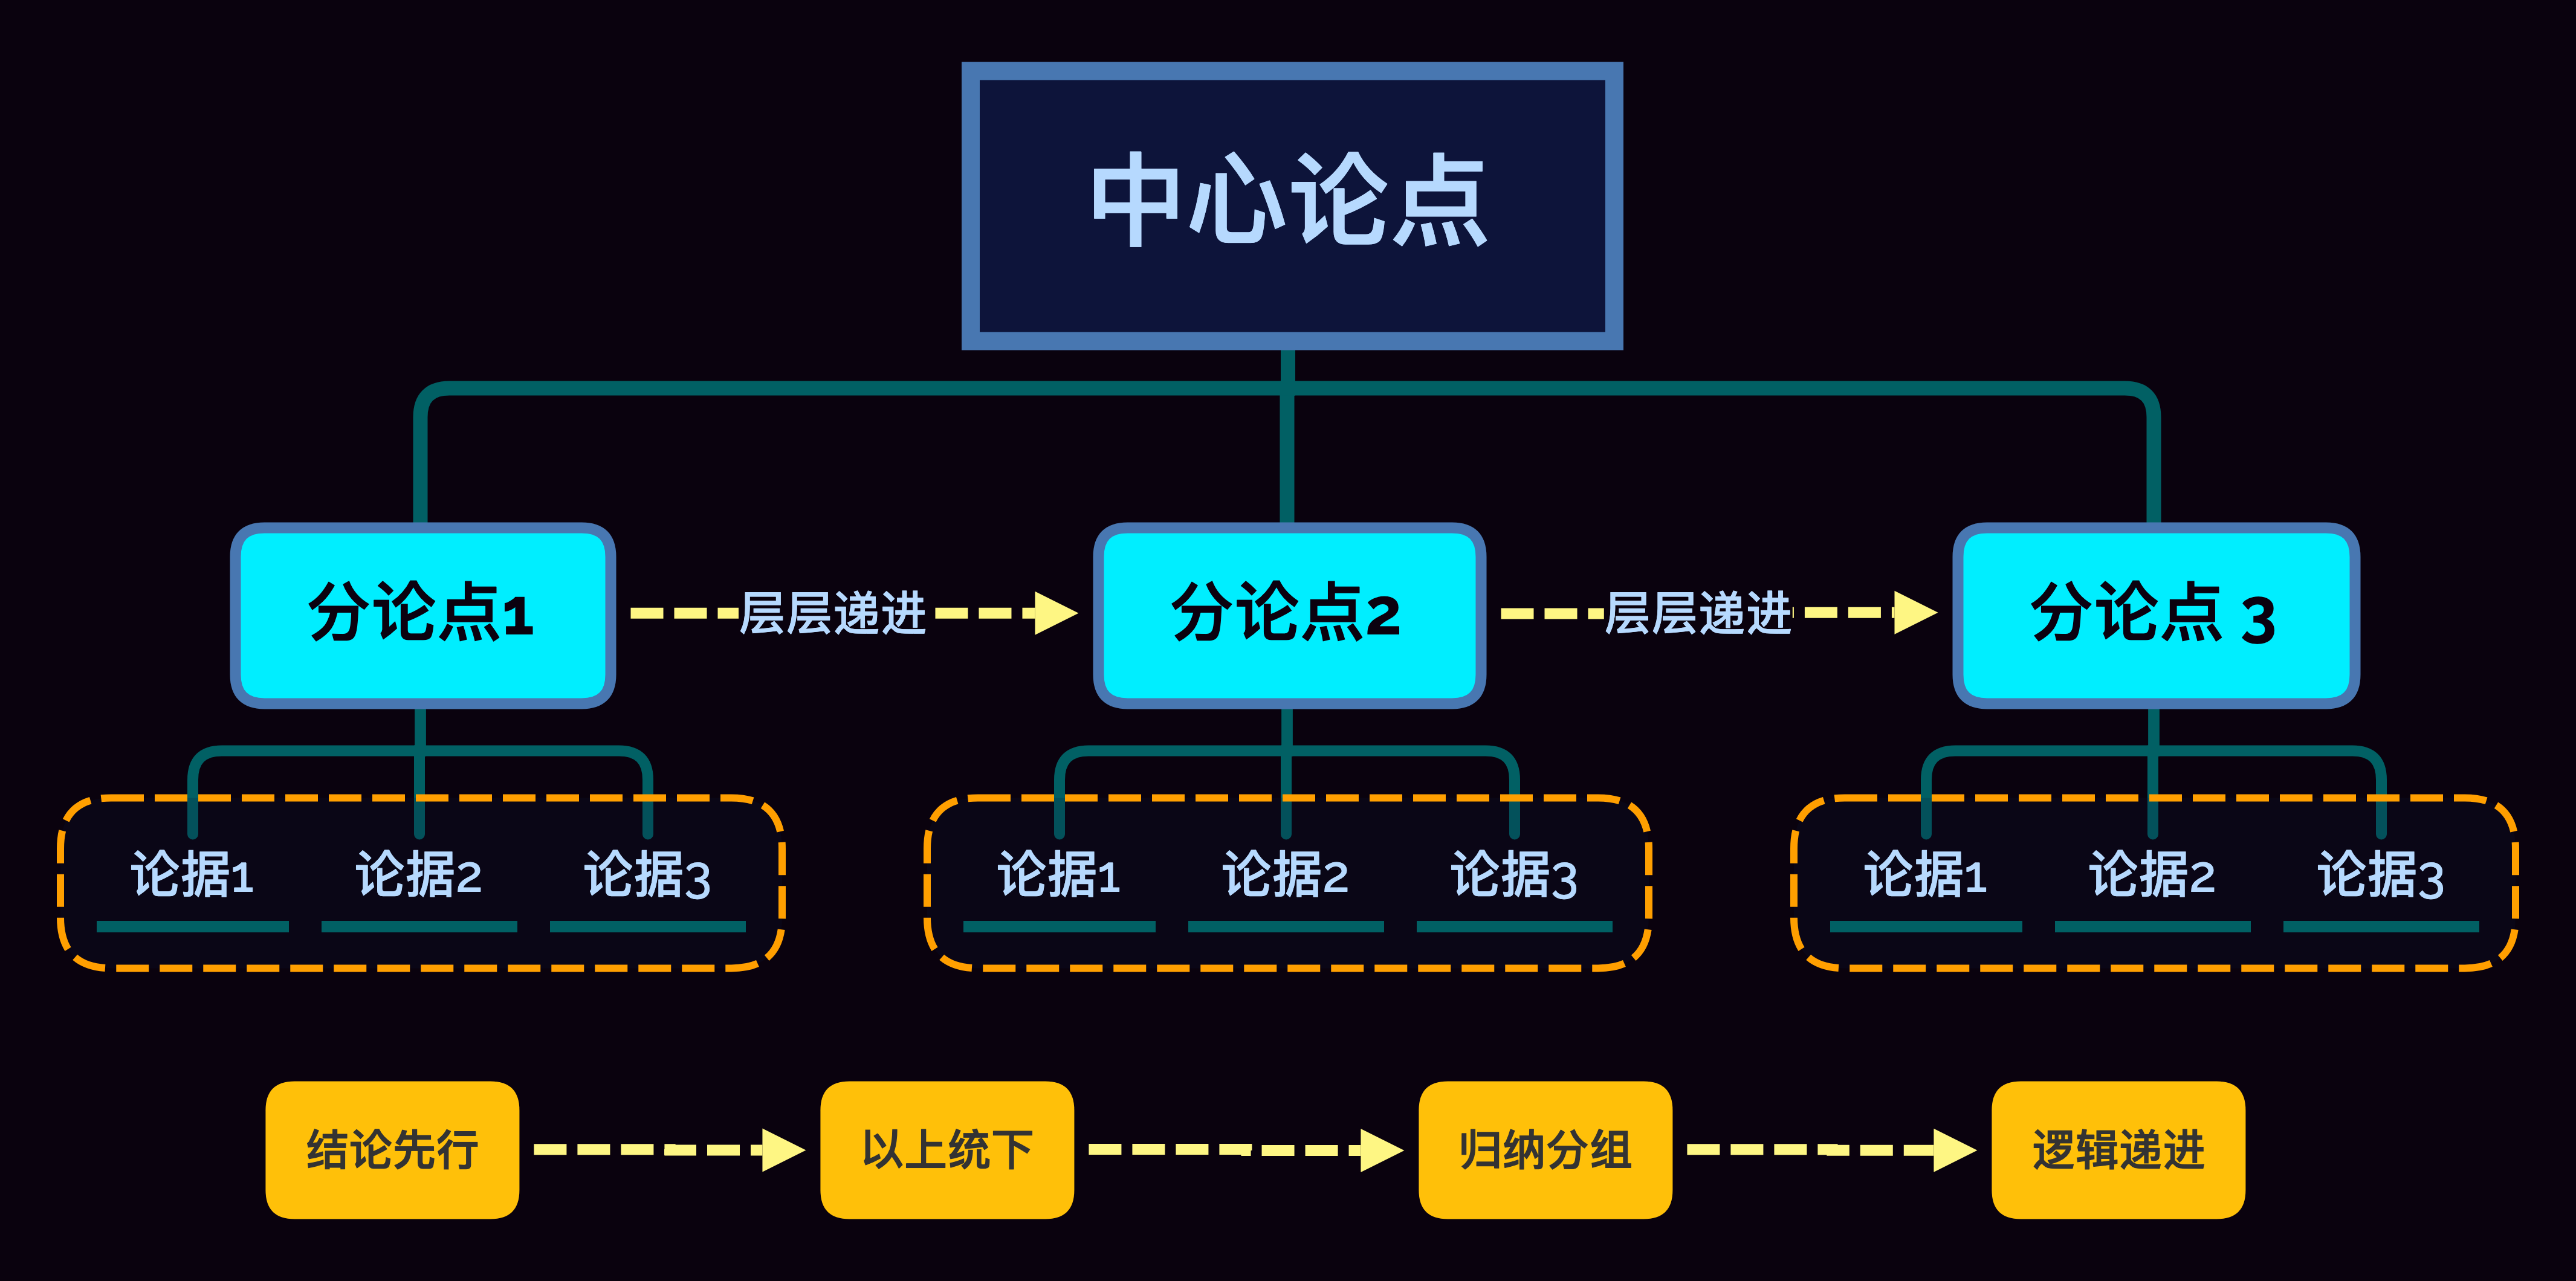
\includegraphics[width=0.80\textwidth]{金字塔法.png}
  \end{center}
  \caption{金字塔法}
\end{figure}
%

除了以上几种常见的思维框架外,还有以下各种常见的思考框架,
可以根据不同的情况,不同的需求灵活运用。
%
\begin{itemize}
  \item STAR法则:情境(Situation)、任务(Task)、行动(Action)、结果(Result)
  \item SMART原则:目标要具体(Specific)、可衡量(Measurable)、
    可达到(Attainable)和其他目标具有相关性(Relevant)、
    具有明确的截止期限(Time-based)
  \item 5W1H原则:原因(Why)、对象(What)、地点(Where)、
    时间(When)、人员(Who)、方法(How)
  \item PDCA模型:通过规划(Plan)、执行(Do)、查核(Check)、
    行动(Act)来达成目标
  \item 4P法:产品(Product)、价格(Price)、渠道(Place)、
    促销(Promotion)
  \item AIDMA法则:A(Attention)引起注意、I (Interest)产生兴趣、
    D(Desire)培养欲望、M(Memory)形成记忆、A(Action)促成行动
\end{itemize}
%
\summary{
  以上即是本次分享的内容。最重要的其实不是具体的思维框架,
  而是如何更好地进行思考。大脑是人体中最性感的器官,
  祝愿大家都能找到思维的乐趣。
}
%
\end{document}
